%\begin{figure}
%  \includegraphics[width=0.25\linewidth]{main_figures/test_figure.png}
%  \caption{A figure.}
%  \label{fig:test_fig}
%\end{figure}
%
%\newpage

In 2001, the first analyses of the draft human genome were published in sister papers in \textit{Nature} and \textit{Science}. The Human Genome Project had been budgeted US\$$3$~billion in 1990; by 2020 the cost of sequencing a human genome had dropped to US\$$1,000$, and a relative paucity of data had given way to abundance\citep{gibbs_human_2020}. Biobanks with data from tens or hundreds of thousands of individuals are becoming commonplace.

Every genome carries both the stories of its ancestors and the basic programming of its bearer's physiology. By identifying patterns across many genomes and their associated data, we can infer their histories and study distributions of biomedical traits. The complexities of human history and society, to say nothing of the complexities of biology itself, ensure that this is a non-trivial task.

With each genome spanning $3$~billion base pairs, any mathematical investigation is high-dimensional. This thesis explores applications of dimensionality reduction to population genetic data, focusing on uniform manifold approximation and projection (UMAP), a method of topological data analysis.

This thesis is organized into three chapters that have been published as stand-alone manuscripts. In \hyperref[chap:chapter1]{Chapter~1} we apply UMAP to human genetic data for the first time. We use genotype data from three biobanks, generating visualizations and observing patterns in relatedness, demographic histories, geographic distribution, phenotype distributions, and other phenomena. In \hyperref[chap:chapter2]{Chapter~2} we review the applications of UMAP in other human genetic datasets, such as different biobanks or other types of genetic data (e.g. structural variants). Finally, in \hyperref[chap:chapter3]{Chapter~3} we formalize a methodology to use UMAP in higher dimensions ($n \ge 3$) and extract clusters.

% high-level concepts?
% shape of data
% population structure
% complexity and interrelatedness

\section{Genetic diversity}

The human genome spans over $3$~billion nucleobase pairs organized across $23$ pairs of chromosomes---$22$ pairs of autosomes and one pair of sex chromosomes---with some DNA present in mitochondria (mtDNA). The human genome is diploid (i.e. paired) with one set of chromosomes coming from each parent via their gametes; these chromosomes are created through the process of meiotic recombination, in which the chromosomes of grandparents are aligned, cross over, and recombine. Along with mutation, recombination generates diversity. Approximately $99.9\%$ of DNA shared between humans is identical, with genetic variants (alleles) arising through mutations. Single nucleotide polymorphisms (SNPs) are relatively common variants, usually defined as having a frequency above $1\%$.

Variants that lie along the same chromosome and are not broken up through recombination are co-inherited and are linked. The block of allelic states along a DNA molecule is referred to as a haplotype, and when the same variants exist between two individuals, they are said to be identical by state (IBS). If the shared variant is inherited from a common ancestor without recombination, they are also said to be identical by descent (IBD); alleles that are IBS are typically IBD, with rare exceptions. Alleles that are physically closer are more likely to be inherited together, and those that appear together more often than expected at random are said to be in linkage disequilibrium (LD). Combining two haplotypes gives a diploid genotype, and assuming free recombination, the theoretical maximum number of possible unique haplotypes is $2^L$, where $L$ is the number of SNPs.

Recombination is not uniformly random. DNA that does not lie in the pseudoautosomal regions (PAR1 and PAR2) of the Y chromosome, as well as mtDNA, does not recombine\citep{jobling_human_2013}. Recombination rates also vary within chromosomes with certain regions known to be hotspots\citep{altemose_map_2017}. Germline mutations may result from copying errors during replication or from spontaneous errors from DNA’s instability or external factors like UV radiation. Whole genome sequencing pedigree-based studies estimate the overall mutation rate at about $10^{-8}$ per base pair per generation, though this rate may vary depending on the mechanistic source of the mutation\citep{segurel_determinants_2014}.

\subsection{Population structure}

% what does structure *look* like?

In aggregate, patterns will form in the distributions of alleles; these patterns are known as population structure. Though genetic diversity is random in principle, the distributions of variants are shaped by environments and events. Phenomena like migrations, population bottlenecks, and non-random mating contribute to the distribution of alleles.

Why is genetic variation not fully random? How do we measure it? What are the processes that we know of? What are some historical examples?

\subsection{Measures of population structure}

\subsubsection{Hardy-Weinberg Equilibrium}

\subsubsection{Fixation index}

\subsubsection{Dimensionality reduction}

\section{Exploratory data analysis}

Though population structure

Exploratory data analysis emphasizes 

\begin{figure}[h!]
\centering
\begin{subfigure}{0.3\textwidth}
    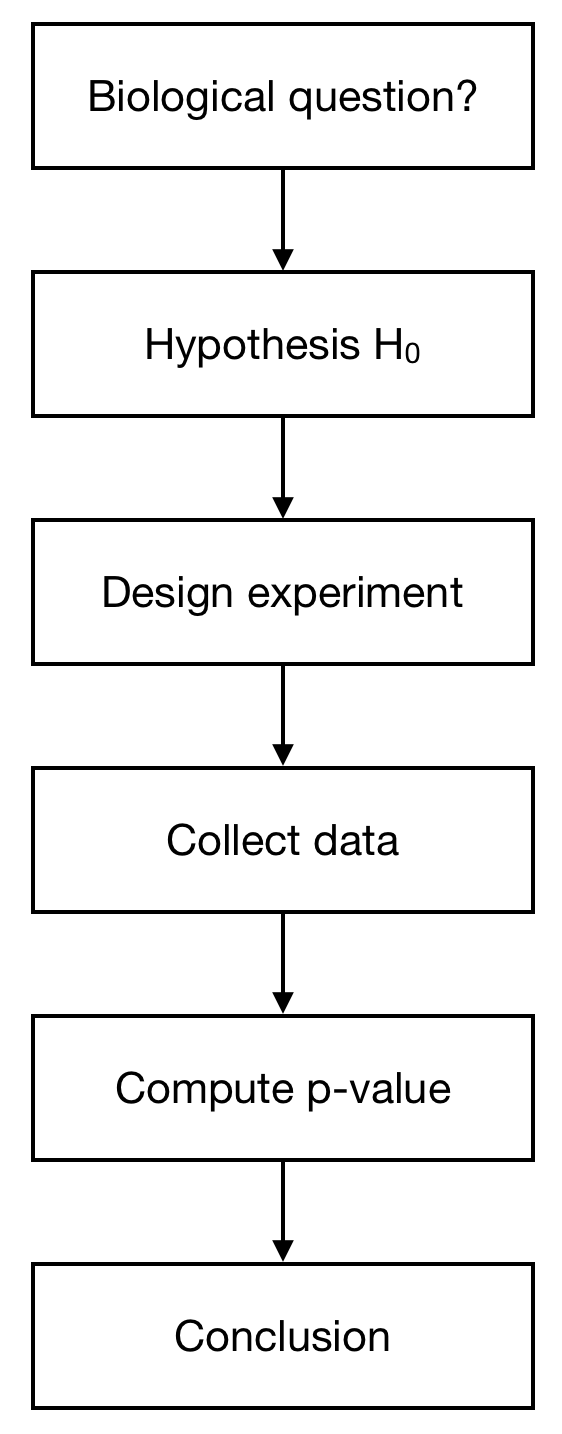
\includegraphics[height=0.5\textheight]{main_figures/intro/fisher_paradigm.png}
    \caption{Fisher's paradigm.}
    \label{fig:fisher}
\end{subfigure}
\hfill
\begin{subfigure}{0.65\textwidth}
    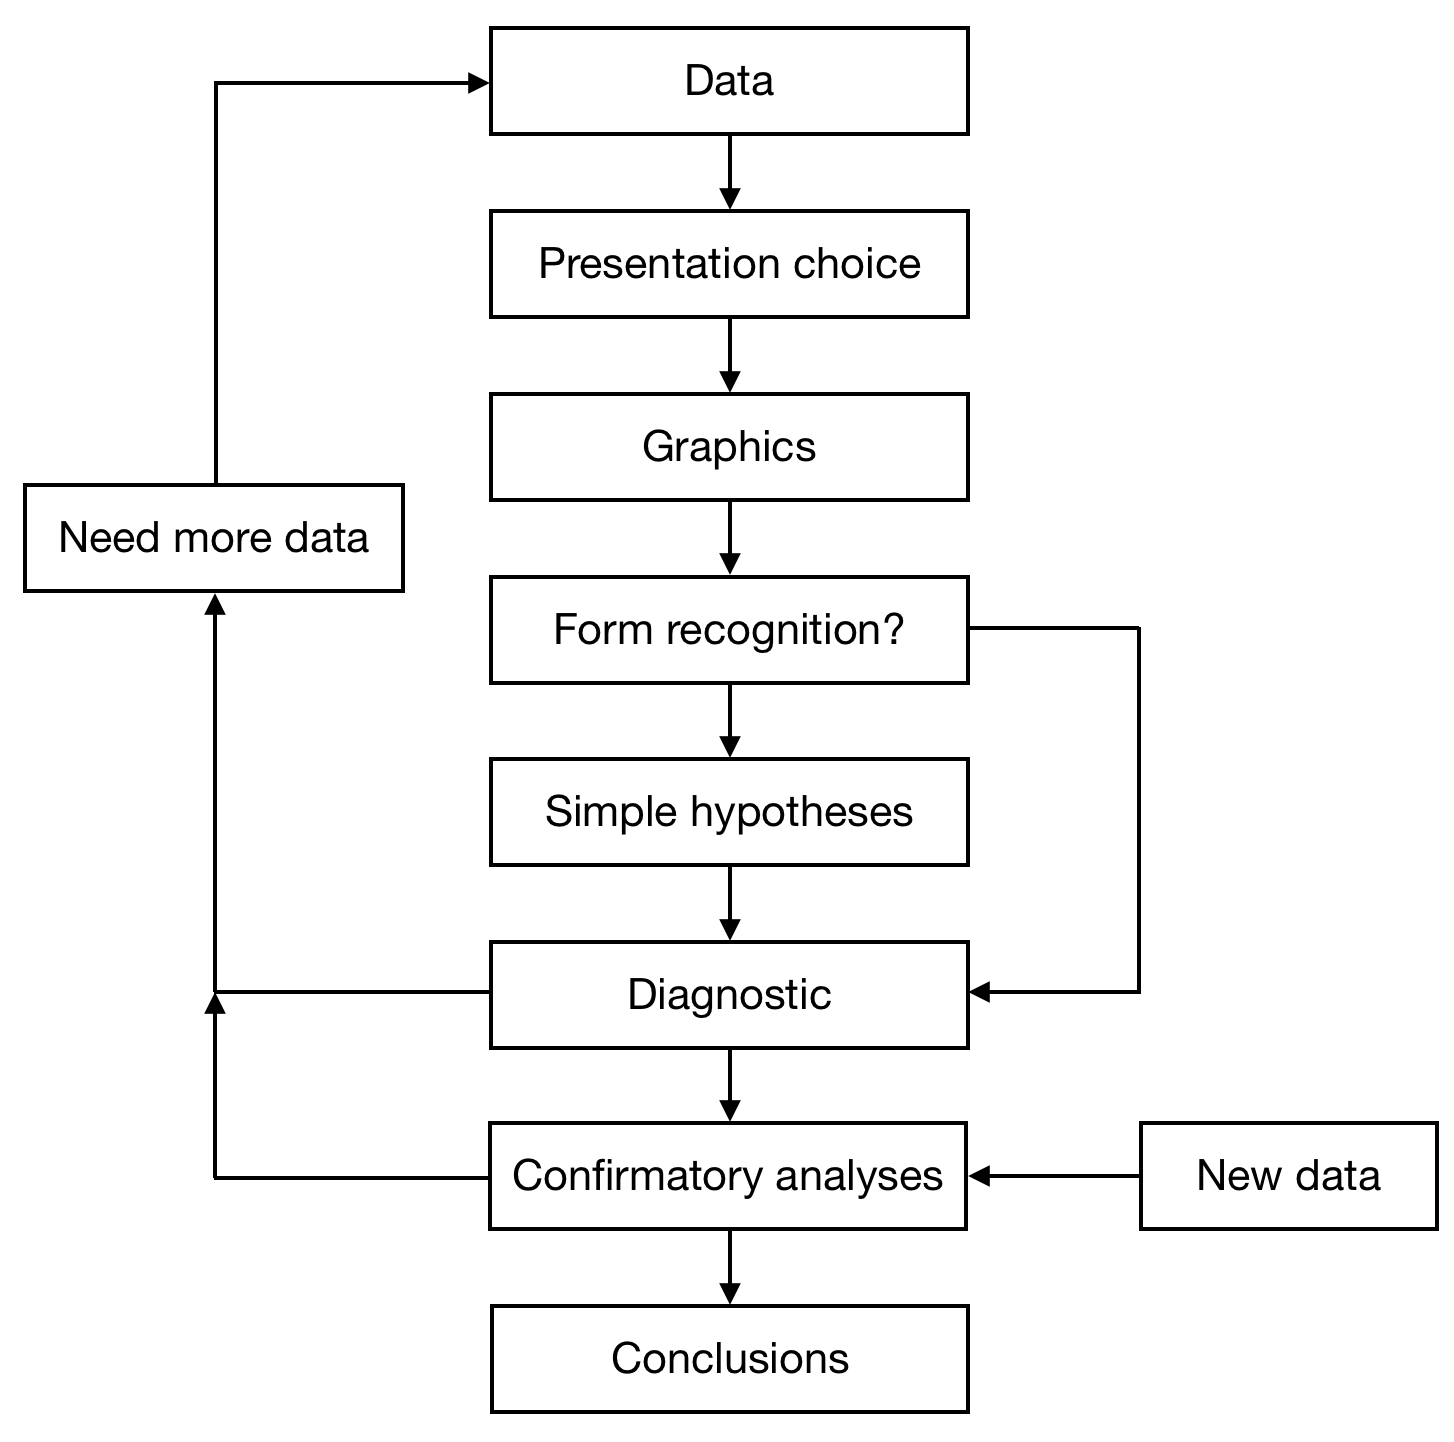
\includegraphics[height=0.5\textheight]{main_figures/intro/tukey_paradigm.png}
    \caption{Tukey's paradigm.}
    \label{fig:tukey}
\end{subfigure}
\caption{\textbf{Contrasting Fisher's paradigm with Tukey's paradigm in biology.} Fisher's paradigm (left) takes a sequential approach to data analysis, beginning with a well-defined question and strong assumptions. Tukey's paradigm (right) is iterative, beginning with the data, emphasizing exploratory analysis through visualization, and complemented by confirmatory analyses that are robust and do not rely on complex assumptions\citep{holmes_modern_2019}.}
\label{fig:paradigms}
\end{figure}

%\begin{figure}[h!]
%\centering
%\begin{subfigure}{0.3\textwidth}
%    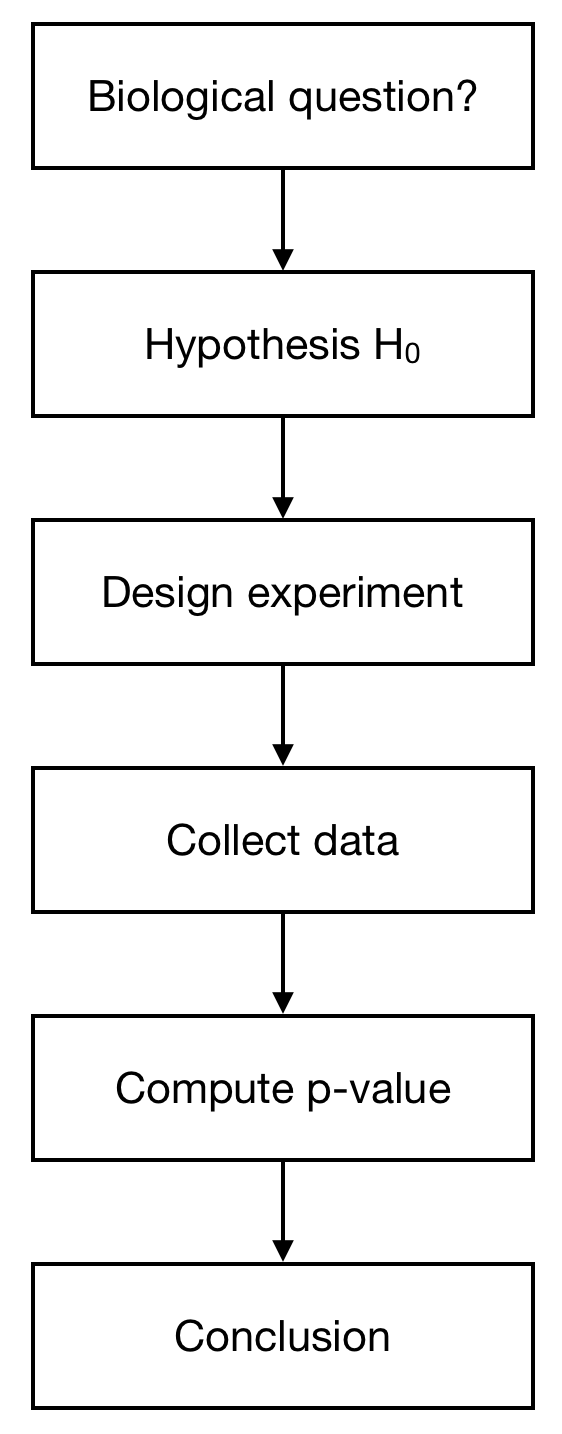
\includegraphics[width=\textwidth]{main_figures/intro/fisher_paradigm.png}
%    \caption{First subfigure.}
%    \label{fig:first}
%\end{subfigure}
%\hfill
%\begin{subfigure}{0.65\textwidth}
%    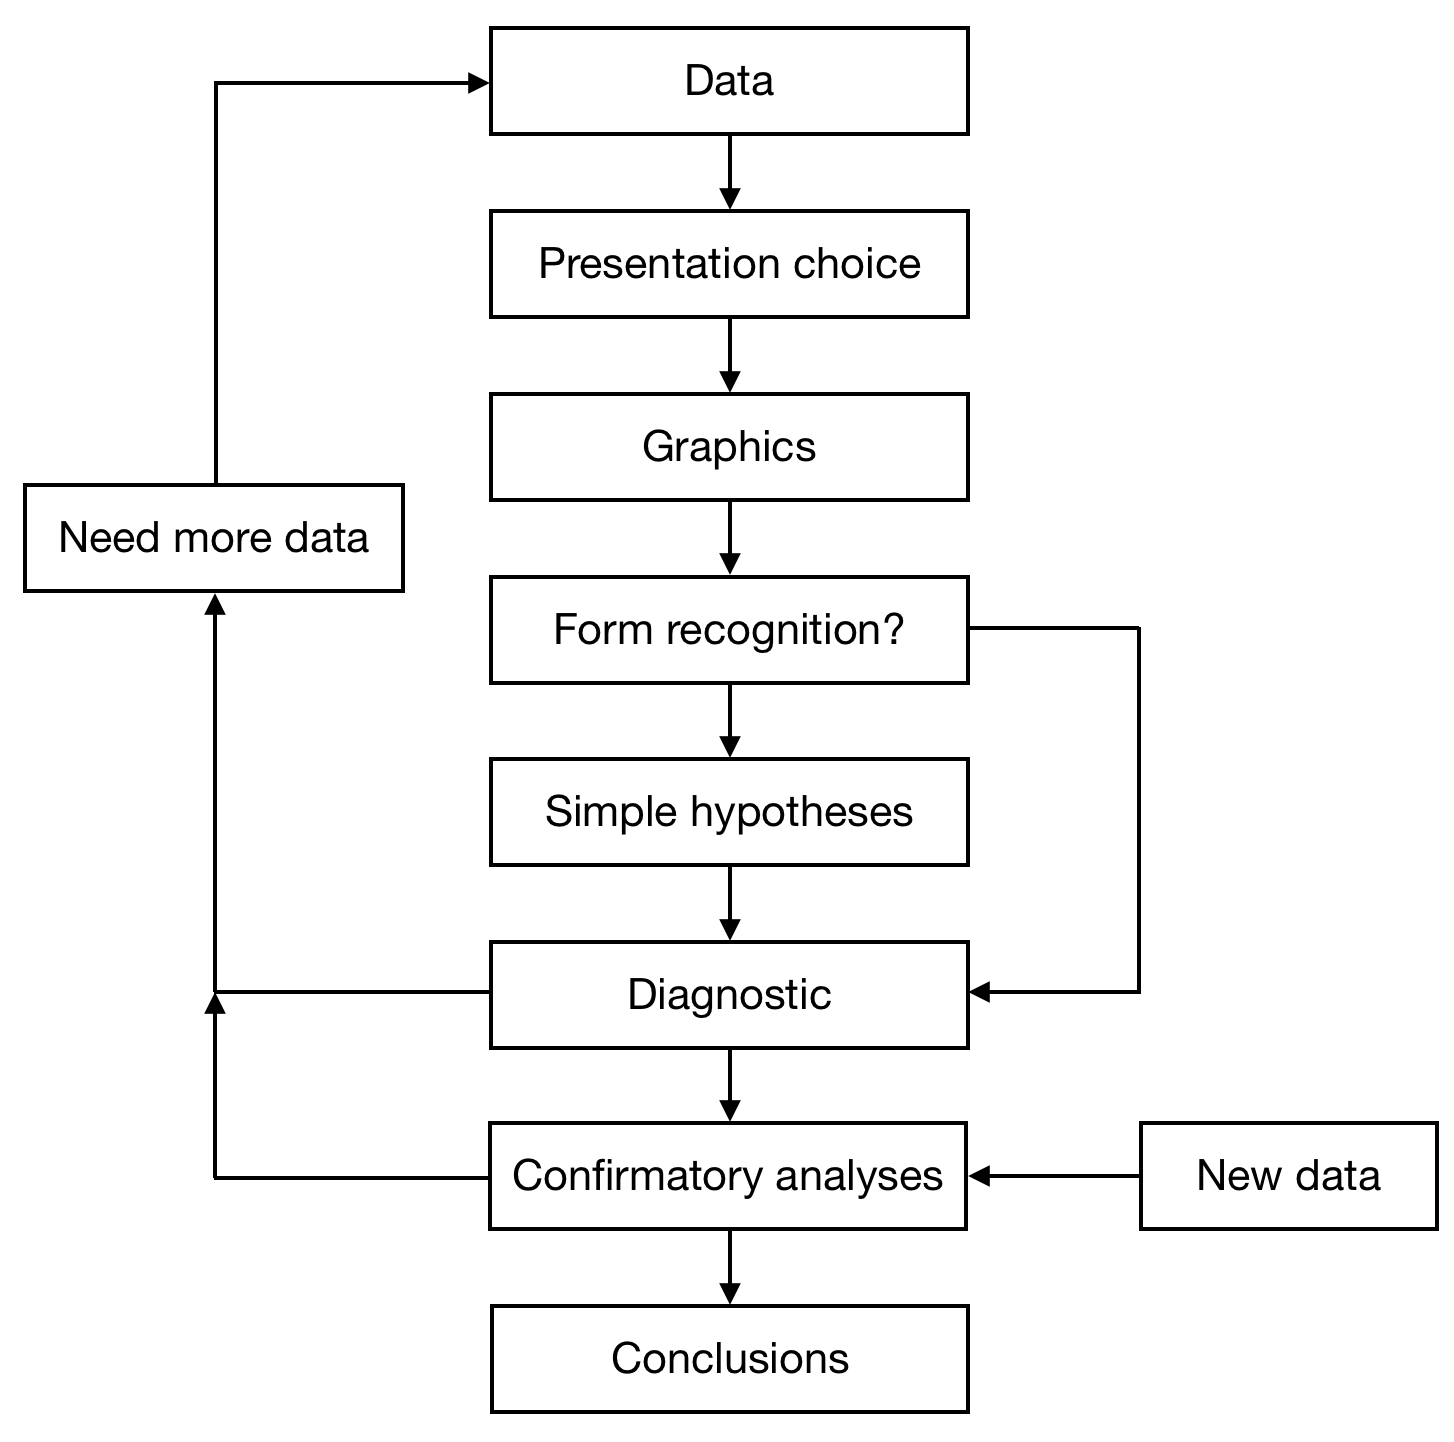
\includegraphics[width=\textwidth]{main_figures/intro/tukey_paradigm.png}
%    \caption{Second subfigure.}
%    \label{fig:second}
%\end{subfigure}
%        
%\caption{Subreferences in \LaTeX.}
%\label{fig:figures}
%\end{figure}

\subsection{Topology and the shape of data}

\subsection{Visualization}

\section{Data}

This research makes use of data from four biobanks. We focus on genotype data coded as the number of non-reference alleles. Given a set of $L$ SNPs for $N$ individuals, the genotype matrix $G$ is:

$$
G = \begin{bmatrix} 
    g_{11} & g_{12} & \dots g_{1L} \\
    \vdots & \ddots & \\
    g_{N1} &        & g_{NL} 
    \end{bmatrix}
    
\text{ where } g_{ij}\text{ is the number of non-reference alleles for individual } i \text{ at locus } j.
$$

\subsection{The 1000 Genomes Project}

The 1000 Genomes Project (1KGP) is a publicly available data set of genetic data sampled from many populations from around the world\citep{global_2015}. We used $3,450$ genotypes from the Affy 6.0 platform sampled from $26$  populations. The populations sizes are roughly similar, with between $104$ to $183$ in each group.

\subsection{CARTaGENE}

CARTaGENE (CaG) is a cohort of residents of Qu\'{e}bec with genotype data for $29,337$ participants, who were recruited using registration data from the R\'{e}gie de l’assurance maladie du Qu\'{e}bec (RAMQ), the provincial health authority\citep{awadalla_cohort_2013}. In addition to genetic data, it contains questionnaire health data and demographic information such as country of birth and ethnicity.

\subsection{Health and Retirement Study}

The Health and Retirement Study (HRS) is a cohort of retired American individuals\citep{juster_overview_1995}. We used genotype data from 12,454 individuals from the Health and Retirement Study (HRS), genotyped on the Illumina Human Omni 2.5M platform. The database contains basic demographic data such as age, US Census Bureau region of birth, and race.

\subsection{UK biobank}

The UK biobank (UKB) is a cohort of individuals living in the United Kingdom who were recruited by inviting those registered with the National Health Service (NHS)\citep{sudlow_uk_2015}. It contains the genotypes from $488,377$ participants as well as detailed health data, phenotypic measures, geographic coordinates, and sociodemographic information such as ethnic background.

%\section{Methods}

%\subsection{PCA}

%\subsection{UMAP}

%\subsection{HDBSCAN(\texorpdfstring{$\hat{\epsilon}$}{f})}
% the {f} here doesn't do anything, but we need a text character for compilation

%\subsection{Genomic tools}